
\chapter{Segmentation}

Segmentation of medical images is a challenging task. A myriad of
different methods have been proposed and implemented in recent
years. In spite of the huge effort invested in this problem, there is
no single approach that could generally solve the problem of
segmentation for the large variety of image modalities existing today.

The most effective segmentation algorithms are obtained by carefully
customizing combinations of components. The parameters of these components are
tuned for the characteristics of the image modality used as input and the
features of the anatomical structure to be segmented. 

The Insight toolkit provides a basic set of algorithms that can be used to
develop and customize a full segmentation application. Some of the most
commonly used segmentation components are described in the following sections.


\section{Region Growing}

Region growing algorithms have proven to be a very effective approach for image
segmentation. The basic concept of a region growing algorithm is to start from
a seed region that is considered to belong to the object to be segmented. The
pixels neigboring this initial region are evaluated to determine if they could
also be considered part of the object, in which case they are added to the
region. When some of the neighbor pixels are included in the region, other
pixels become new neighbors and hence become candidates to be evaluated and
eventually included in the region. Region growing algorithms vary depending on
the criteria used to decide whether a pixel should be included in the region
or not, the type of neighbor connectivity used on the image grid and the
strategy used for visiting the neighbor pixels.

Several implementations of region growing are available in the
Insight toolkit. This section describes some of the most commonly used.

\subsection{Connected Threshold}

The simplest criterion for including pixels in a growing region is
probably the condition of having intensity values inside a specific
interval.

\label{sec:ConnectedThreshold}
\ifitkFullVersion 
\input{ConnectedThresholdImageFilter.tex}
\fi


\subsection{Neighborhood Connected}
\label{sec:NeighborhoodConnectedImageFilter}
\ifitkFullVersion 
\input{NeighborhoodConnectedImageFilter.tex}
\fi



\subsection{Confidence Connected}
\label{sec:ConfidenceConnected}
\ifitkFullVersion 
\input{ConfidenceConnected.tex}
\fi


\subsection{Isolated Connected}
\label{sec:IsolatedConnected}
\ifitkFullVersion 
\input{IsolatedConnectedImageFilter.tex}
\fi


\subsection{Confidence Connected in Vector Images}
\label{sec:VectorConfidenceConnected}
\ifitkFullVersion 
\input{VectorConfidenceConnected.tex}
\fi


\section{Segmentation Based on Watersheds}
\label{sec:WatershedSegmentation}
\ifitkFullVersion 
\input WatershedSegmentation.tex
\fi


\section{Level Sets Segmentation}
\label{sec:LevelSetsSegmentation}
\ifitkFullVersion 
%%%%%%%%%%%%%%%%%%%%%%%%%%%%%%%%%%%%%%%%%%%%%%%%%%%%%%%%%%%%%%%%%%%%%%%%
%
%
%     This file is included from the file   Segmentation.tex
% 
%     Section tag and label are placed in this top file.
%
%
%
%%%%%%%%%%%%%%%%%%%%%%%%%%%%%%%%%%%%%%%%%%%%%%%%%%%%%%%%%%%%%%%%%%%%%%%%



\itkpiccaption[Zero Set Concept]{Concept of Zero Set in a Level Set.\label{fig:LevelSetZeroSet}}
\parpic(9cm,6cm)[r]{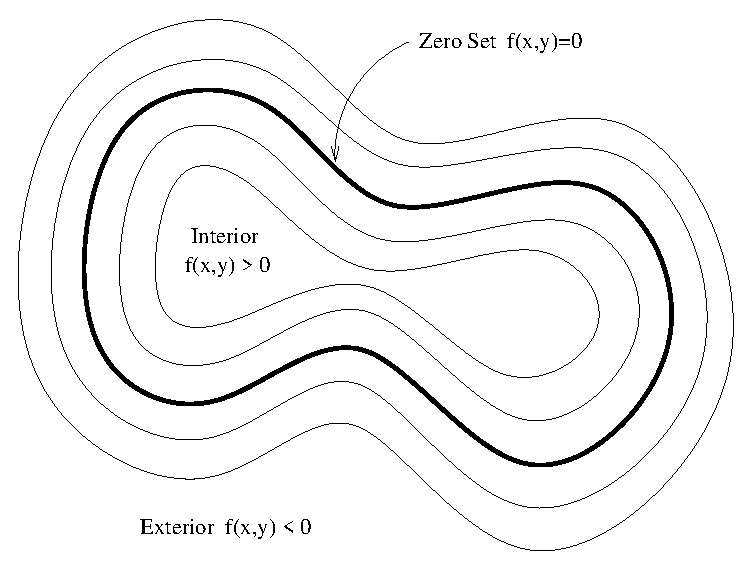
\includegraphics[width=8cm]{LevelSetZeroSet.eps}}

The paradigm of Level Set is a numerical method for tracking the evolution of
contours and surfaces. Instead of manipulating the contour directly, the
contour is embedded as the zero level set of a higher dimensional function
called the level-set function, $\psi(\bf{X},t)$. The level-set function is then
evolved under the control of a differential equation.  At any time, the evolving
contour can be obtained by extracting the zero level-set $\Gamma(\bf(X),t) =
\{\psi(\bf{X},t) = 0\}$ from the output.  The main advantages of using level
sets is that arbitrarily complex shapes can be modeled and topological
changes such as merging and splitting are handled implicitly. 

Level sets can be used for image segmentation by using image-based features such
as mean intensity, gradient and edges in the governering differential equation. 
In a typical approach, a contour is initialized by a user and is then evolved 
until it fits the form of an anatomical structure in the image. 
Many different implementations and variants of this basic concept have been
published in the literature. An overview of the field has been made by Sethian
\cite{Sethian1996}. 

The following sections introduce practical examples of some
of the Level Set segmentation methods available in ITK.  The remainder of this
section describes features common to all of these filters except the
\code{FastMarchingImageFilter}, which is derived from a different code
framework.  Understanding these features will aid in using the filters
more effectively.

Each filter makes use of a generic level-set equation to compute the update to
the solution $\psi$ of the partial differential equation.

\begin{equation}
\label{eqn:LevelSetEquation}
\frac{d}{dt}\psi = -\alpha \mathbf{A}(\mathbf{x})\cdot\nabla\psi - \beta
  P(\mathbf{x})\mid\nabla\psi\mid + \gamma Z(\mathbf{x})\kappa
\end{equation}
 
where $\mathbf{A}$ is an advection term, $P$ is a propagation (expansion) term,
and $Z$ is a spatial modifier term for the mean curvature $\kappa$.  The scalar
constants $\alpha$, $\beta$, and $\gamma$ weight the relative influence of
each of the terms on the movement of the interface.  A segmentation filter may
use all of these terms in its calculations, or it may omit one or more terms.
If a term is left out of the equation, then setting the corresponding scalar
constant weighting will have no effect.

All of the level-set based segmentation filters \emph{must} operate with
floating point precision to produce valid results.  The third, optional
template parameter is the \emph{numerical type} used for calculations and as
the output image pixel type.  The numerical type is \code{float} by default,
but can be changed to \code{double} for extra precision.  A user-defined,
signed floating point type that defines all of the necessary arithmetic
operators and has sufficient precision is also a valid choice.  You should not
use types such as \code{int} or \code{unsigned char} for the numerical
parameter.  If the input image pixel types do not match the numerical type,
those inputs will be cast to an image of appropriate type when the filter is
executed.

Most filters require two images as input, an initial model $\psi(\bf{X}, t=0)$,
and a \emph{feature image}, which is either the image you wish to segment or
some preprocessed version therof.  You must specify the isovalue that
represents the surface $\Gamma$ in your initial model. The single image output of
each filter is the function $\psi$ at the final time step.  It is important to
note that the contour representing the surface $\Gamma$ is the zero level-set
of the output image, and not the isovalue you specified for the initial model.
To represent $\Gamma$ using the original isovalue, simply add that value back
to the output.

The solution $\Gamma$ is calculated to subpixel precision.  The best discrete
approximation of the surface is therefore the set of grid positions closest to
the zero-crossings in the image, as shown in
figure~\ref{fig:LevelSetSegmentationFigure1}.  The
\code{itk::ZeroCrossingImageFilter} operates by finding exactly those grid 
positions and can be used to extract the surface. 

\begin{figure}
\centering
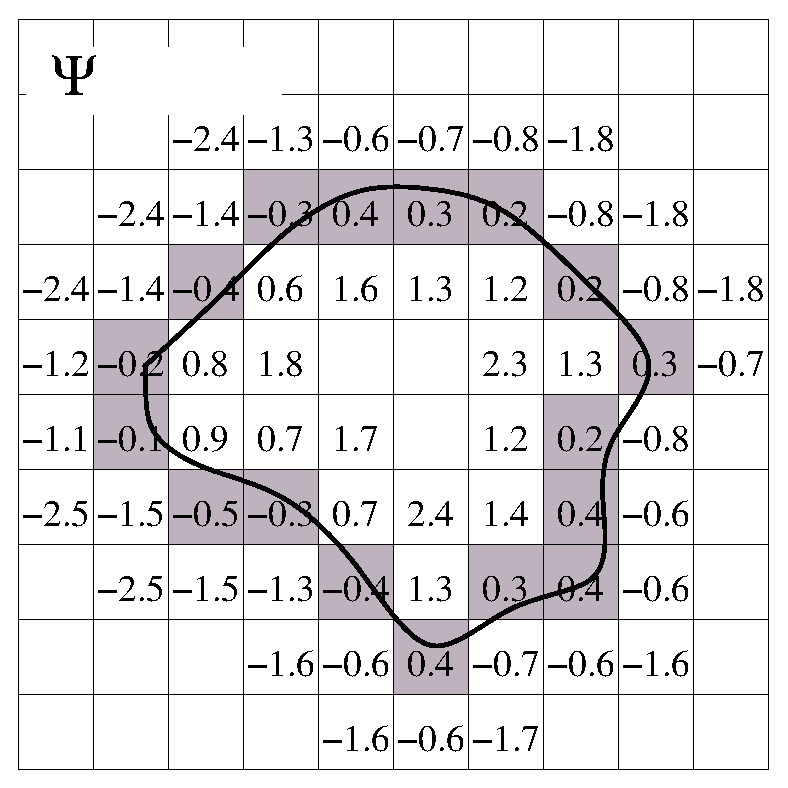
\includegraphics[width=0.4\textwidth]{LevelSetSegmentationFigure1.eps}
\itkcaption[Grid position of the embedded level-set surface.]{The implicit level
set surface $\Gamma$ is the black line superimposed over the image grid.  The location
of the surface is interpolated by the image pixel values.  The grid pixels
closest to the implicit surface are shown in gray. }
\protect\label{fig:LevelSetSegmentationFigure1}
\end{figure}

There are two important considerations when analyzing the processing time for
any particular level-set segmentation task: the surface area of the evolving
interface and the total distance that the surface must travel.  Because the
level-set equations are usually solved only at pixels near the surface (fast
marching methods are an exception), the time taken at each iteration depends on
the number of points on the surface.  This means that as the surface grows, the
solver will slow down proportionally.  Because the surface must evolve slowly
to prevent numerical instabilities in the solution, the distance the surface
must travel in the image dictates the total number of iterations required.

Some level-set techniques are relatively insensitive to initial conditions and are
therefore suitable for region-growing segmentation. Other techniques, like
\code{itk::LaplacianSegmentationLevelSetImageFilter}, can easily become
``stuck'' on image features close to their initialization and should be used
only when a reasonable prior segmentation is available as the initialization.
For best efficiency, your initial model of the surface should be the
best guess possible for the solution.  When extending the example applications
given here to higher dimensional images, for example, you can improve results
and dramatically decrease processing time by using a multi-scale
approach. Start with a downsampled volume and work back to the full resolution
using the results at each intermediate scale as the initialization for the next
scale.


\subsection{Fast Marching Segmentation}
\label{sec:FastMarchingImageFilter}

\ifitkFullVersion
\input{FastMarchingImageFilter.tex}
\fi



\subsection{Shape Detection Segmentation}
\label{sec:ShapeDetectionLevelSetFilter}

\ifitkFullVersion
\input{ShapeDetectionLevelSetFilter.tex}
\fi


\subsection{Geodesic Active Contours Segmentation}
\label{sec:GeodesicActiveContourImageFilter}

\ifitkFullVersion
\input{GeodesicActiveContourImageFilter.tex}
\fi


\subsection{Threshold Level Set Segmentation}
\label{sec:ThresholdSegmentationLevelSetImageFilter}
\ifitkFullVersion
\input{ThresholdSegmentationLevelSetImageFilter.tex}
\fi

\subsection{Canny-edge Level Set Segmentation}
\label{sec:CannySegmentationLevelSetImageFilter}
\ifitkFullVersion
\input{CannySegmentationLevelSetImageFilter.tex}
\fi

\subsection{Laplacian Level Set Segmentation}
\label{sec:LaplacianSegmentationLevelSetImageFilter}
\ifitkFullVersion
\input{LaplacianSegmentationLevelSetImageFilter.tex}
\fi



\fi


\section{Hybrid Methods} 
\label{sec:HybridSegmentationMethods}

\ifitkFullVersion 
%%%%%%%%%%%%%%%%%%%%%%%%%%%%%%%%%%%%%%%%%%%%%%%%%%%%%%%%%%%%%%%%%%%%%%%%
%
%
%     This file is included from the file   Segmentation.tex
% 
%     Section tag and label are placed in this top file.
%
%
%
%%%%%%%%%%%%%%%%%%%%%%%%%%%%%%%%%%%%%%%%%%%%%%%%%%%%%%%%%%%%%%%%%%%%%%%%

\subsection{Introduction}
\label{sec:HybridSegmentationIntroduction}


Hybrid methods for automated segmentation of radiological patient data and the 
Visible Human data integrate boundary-based and region-based segmentation methods 
that amplify the strength but reduces the weakness of both approaches.The novelty 
comes from combining a region-based segmentation methods, the fuzzy connectedness 
and Voronoi Diagram classification with a boundary-based deformable model 
segmentation, to develop hybrid methods that yield high precision, accuracy and 
efficiency.The synergy between fundamentally different methodologies tends to 
result in robustness and higher segmentation quality. We built Hybrid Segmentation 
Engine,  Figure \ref{fig:ComponentsofaHybridSegmentationApproach}, that consists of modules 
representating component segmentation methods (itk filters). We can derive a variety 
of hybrid segmentation methods from the modules. It should be noted that under Fuzzy 
Connectedness module and Deformable Models module, we checked in into the itk a number 
of filters in each of the categories, respectively. Below, we decribe two examples of
hybrid segmentation methods, derived from the Hybrid segmentation Engine: Hybrid 
Method 1: Integration of Fuzzy Connectedness and Voronoi Diagram Classification;
Hybrid Method 2: Integration of Gibbs prior and Deformable Models.
Details on the concepts behind those methods have been discussed in the
literature
\cite{Angelini2002,Udupa2002,Jin2002,Imielinska2001,Imielinska2000a,Imielinska2000b}



\subsection{FuzzyConectedness and VoronoiDiagramClassification}
\label{sec:HybridMethod1}

In this section, we present a hybrid segmentation method that requires minimal
manual initialization, where we integrate the fuzzy connectedness segmentation
and Voronoi Diagram Classification. We start with fuzzy connectedness filter
to generate a sample of tissue from a region to be segmented. From the sample,
we derive automatically, homogeneity statistics that constitute homogeneity
operator to be used in the next stage of the method. The output of the fuzzy 
connectedness filter is used as a prior for the Voronoi Diagram Classification 
filter that performs iterative subdivision and classification of the segmented
image that results in an estimation of the boundary. The output of this filter
is a 3D binary image that can be used to display the 3D result of the
segmentation, or passed to another filter (e.g. Deformable Model) for further
improvement of the final segmentation. Details describing the concepts behind those methods 
have been published in
\cite{Angelini2002,Udupa2002,Jin2002,Imielinska2001,Imielinska2000a,Imielinska2000b}

In Figure \ref{fig:UMLClassDiagramoftherFuzzyConnectednessFilter}, we describe 
base class for simple fuzzy connectedness segmentation. This method is non-scale 
based, non-iterative and requires only one seed to initialize it. We define affinity 
between two nearby elements in a image (e.g. pixels, voxels) via a degree of adjacency, 
similarity of their intensity values, and their similarity with the estimated object. 
The closer the elements are and more similar their intensities are, the greater is 
the affinity between them. We compute the strength of a path and fuzzy connectedness 
between each two pixels (voxels) in the segmented image from the fuzzy affinity. 
Computation of fuzzy connectedness value of each pixel (voxel) is implemented
by selecteing a seed point and using dynamic programming. The result constitutes the fuzzy
map. Thresholding of the fuzzy map gives a segmented object that is strongly connected
to the seed point (for more details, see \cite{Udupa1996}). We checked in two fuzzy 
connectedness filters: the itkSimpleFuzzyConnectednessScalarImageFilter that is an
implementation of the fuzzy connectedness segmentation of single channel (gray scale) 
image;itkSimpleFuzzyConnectednessRGBImageFilter that is an implementation of fuzzy
connectedness implementation of three-channel (RGB) image. Other classes can be derived 
from the base class by defining other affinity function, and targeting multi-channel
images with and arbitrary number of channels. It has to be noted, that the simple fuzzy 
connectedness filter can be used as a stand-alone segmentation method,
as it is described in the diagram in Figure 
\ref{fig:UMLCollaborationDiagramoftheFuzzyConnectednessFilter}.

In Figure \ref{fig:UMLVoronoiSegmentationClassFilter} we present base class for
Voronoi Diagram Clasification. We initialize the method with a number of random
seed points and compute Voronoi Diagram over the segmented 2D image. Each
Voronoi region, in teh subdivision, is classified as internal or external,
based on the homogeneity operator derived from the fuzzy connectedness
algorithm.  We define boundary regions as the external regions that are
adjacent to the internal regions.  We subdivide further the boundary regions
by adding seed points to the regions. We converge to the final segmentation
using simple stopping criterium (for details, see \cite{Imielinska2001}). We
implemneted two Voronoi Diagram filters: the
itkVoronoiSegmentationImageFilter that is dedicated to process single channel
(gray scale) images; the itkVoronoiSegmentationRGBImageFilter that segments
three-channel (RGB) images. Other classes can be derivedfrom the base class
by defining other homogeneity measurements, and targeting multichannel images
with and arbitrary number of channels.  The other classes that are used for
computing 2D Voronoi Diagram, are shown in Figure
\ref{fig:UMLClassesforImplementationofVoronoiDiagramFilter}. We note that the
Voronoi Diagram Filter can be used as a stand-alone segmentation method, as
it is depicted in Figure
\ref{fig:UMLCollaborationDiagramoftheVoronoiSegmentationFilter}.

 We present in Figure \ref{fig:UMLHybridMethodDiagram1} and Figure
 \ref{fig:UMLHybridMethodDiagram2} diagrams for hybrid segmentation methods
 that integrate: fuzzy connectedness with Voronoi Diagram; and fuzzy
 connectedness, Voronoi Diagram with Deformable Models, respectively.


%%%%%%%%%%%%%%%%%%%%%%%%%%%%%%%%%%%%%%%%%%%%%%%%%%%%%%%%%%%%%%%%%
%
%  Here is an example of how to include diagram in a figure
%
%  The file HybridSegmentationDiagram1.fig should be in the "Art"
%  directory. CMake will convert it to EPS before running latex. 
%
%%%%%%%%%%%%%%%%%%%%%%%%%%%%%%%%%%%%%%%%%%%%%%%%%%%%%%%%%%%%%%%%%

\begin{figure}
\center
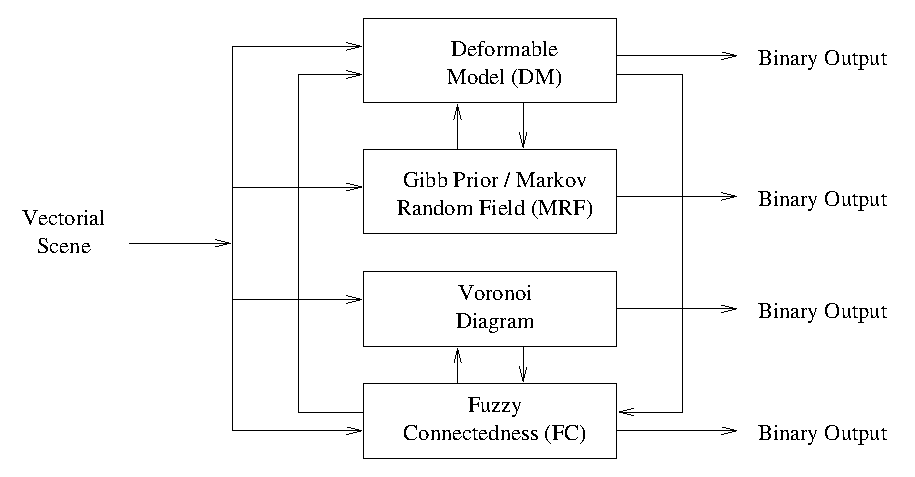
\includegraphics[width=14cm]{HybridSegmentationEngine1.eps}
\caption{Hybrid Segmentation Engine}
\label{fig:ComponentsofaHybridSegmentationApproach}
\end{figure}


\begin{figure}
\center
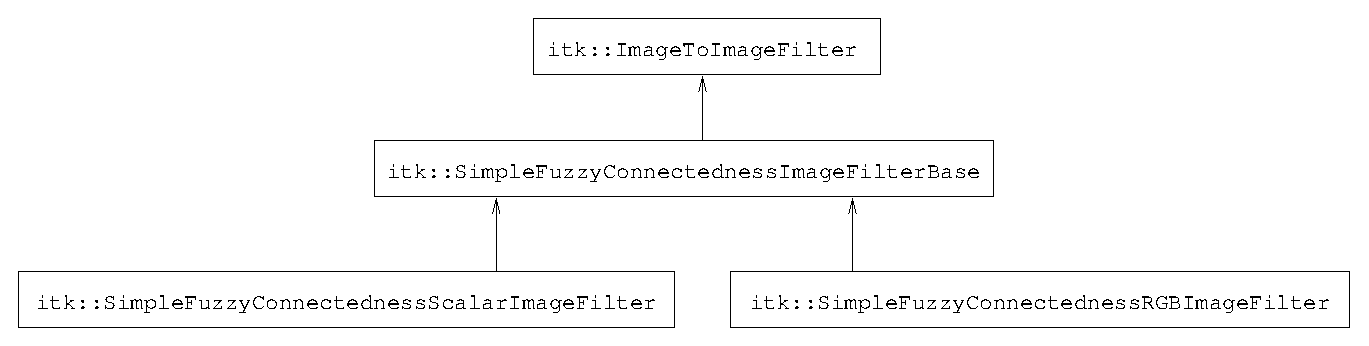
\includegraphics[width=14cm]{FuzzyConnectednessClassDiagram1.eps}
\caption{Diagram of the FuzzyConnectedness filter}
\label{fig:UMLClassDiagramoftherFuzzyConnectednessFilter}
\end{figure}


\begin{figure}
\center
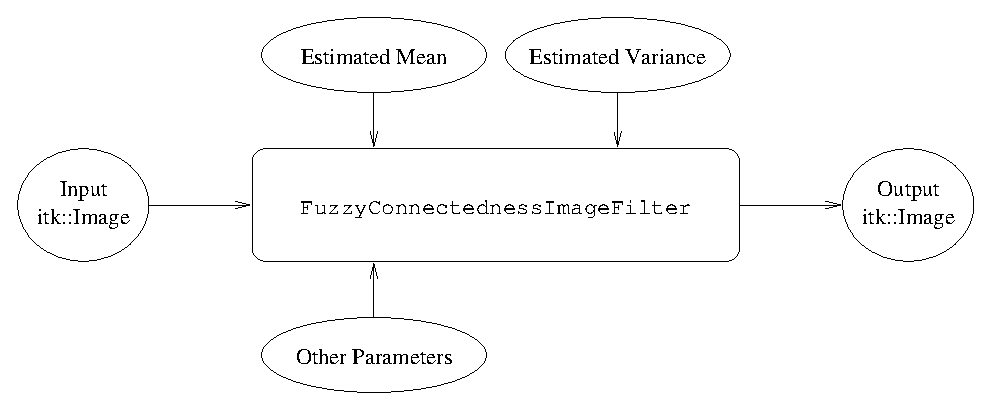
\includegraphics[width=14cm]{FuzzyConnectednessCollaborationDiagram1.eps}
\caption{Diagram Of Stand-Alone Fuzzy Connectedness Segmentation}
\label{fig:UMLCollaborationDiagramoftheFuzzyConnectednessFilter}
\end{figure}

\begin{figure}
\center
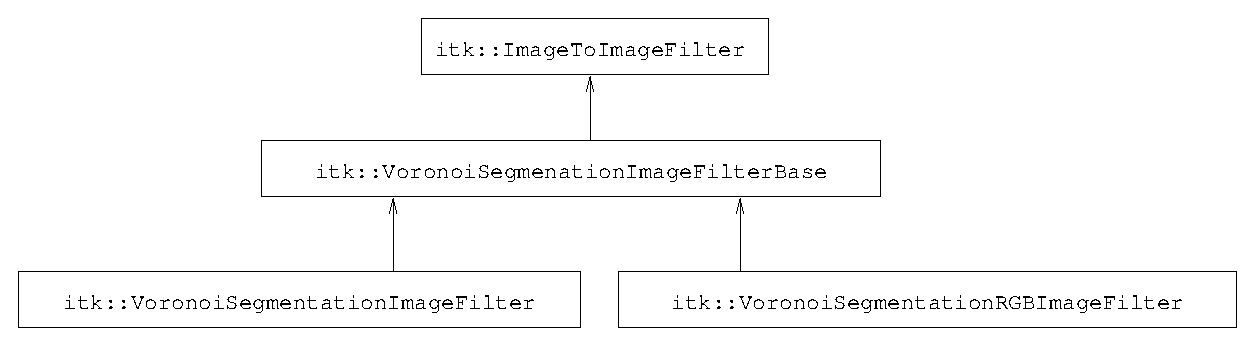
\includegraphics[width=14cm]{VoronoiSegmentationClassDiagram1.eps}
\caption{Diagram of the Voronoi Diagram Classification filter}
\label{fig:UMLVoronoiSegmentationClassFilter}
\end{figure}

\begin{figure}
\center
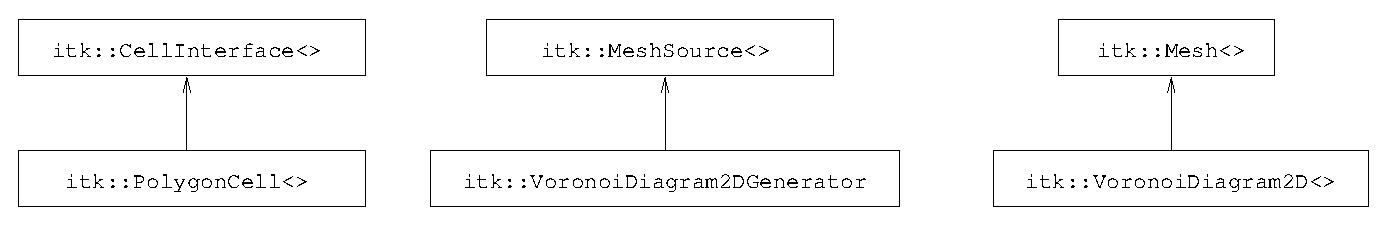
\includegraphics[width=14cm]{VoronoiSegmentationCollaborationDiagram1.eps}
\caption{Classes for Implementation of Voronoi Diagram Filter}
\label{fig:UMLClassesforImplementationofVoronoiDiagramFilter}
\end{figure}


\begin{figure}
\center
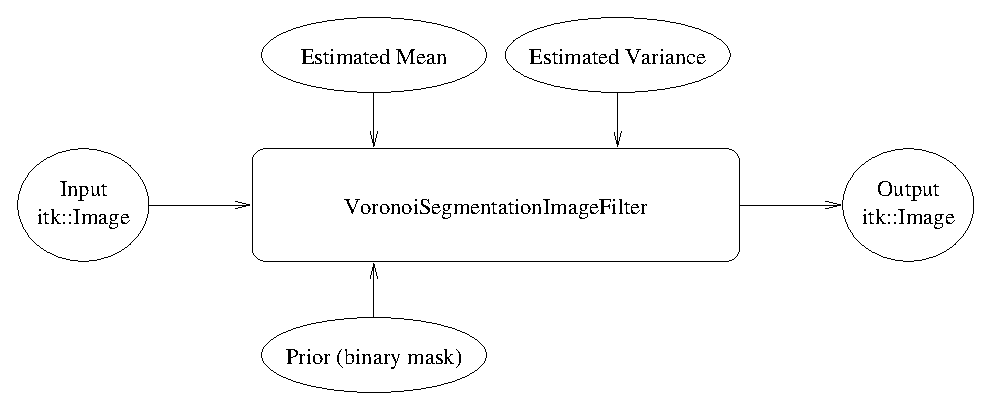
\includegraphics[width=14cm]{VoronoiSegmentationCollaborationDiagram2.eps}
\caption{Diagram Of Stand-Alone Voronoi Diagram Segmentation}
\label{fig:UMLCollaborationDiagramoftheVoronoiSegmentationFilter}
\end{figure}


\begin{figure}
\center
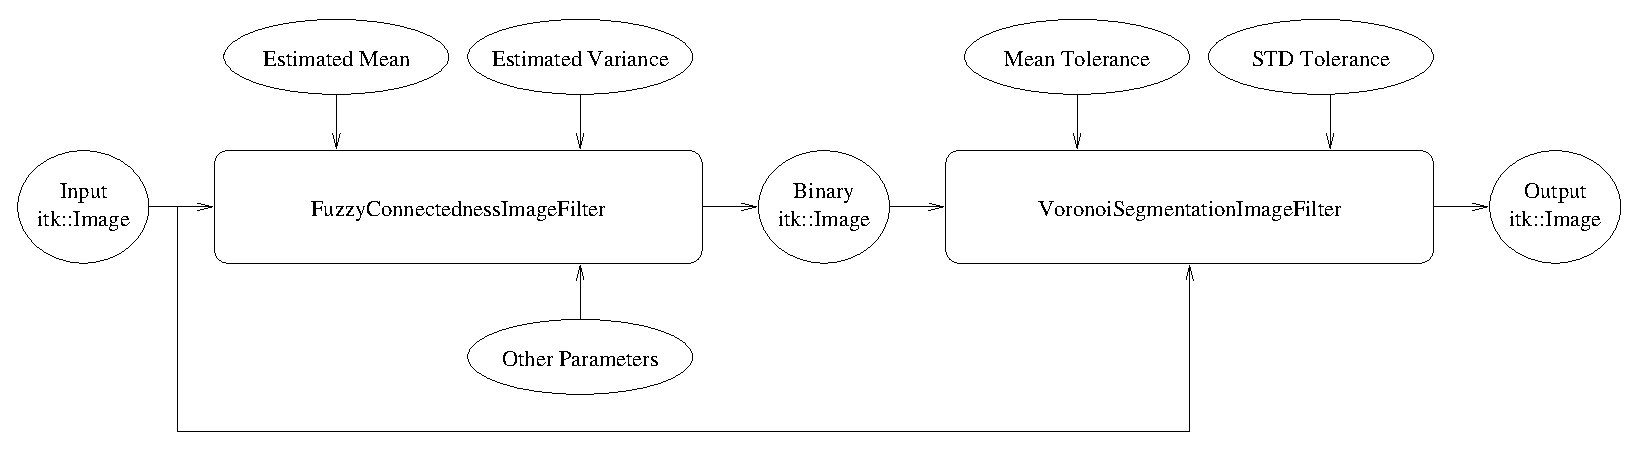
\includegraphics[width=14cm]{FuzzyVoronoiCollaborationDiagram1.eps}
\caption{Integration of Fuzzy Connectedness with Voronoi Diagram Classification}
\label{fig:UMLHybridMethodDiagram1}
\end{figure}

\begin{figure}
\center
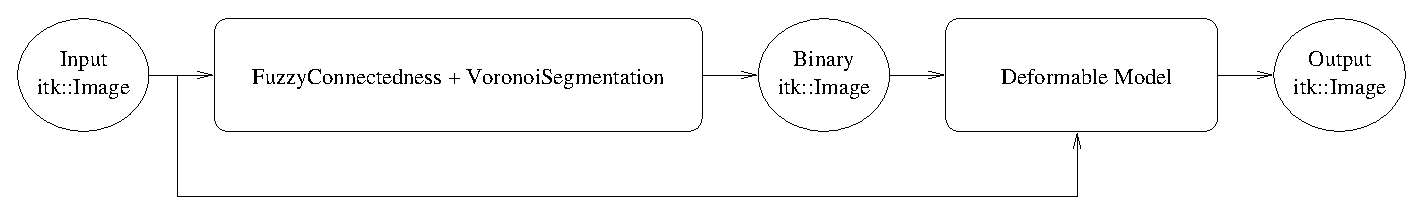
\includegraphics[width=14cm]{FuzzyVoronoiDeformableCollaborationDiagram1.eps}
\caption{Integration of Fuzzy Connectedness, Voronoi Diagram, and Deformable Models}
\label{fig:UMLHybridMethodDiagram2}
\end{figure}



\subsubsection{Example of an Hybrid segmentation Method}
\label{sec:HybridMethod1:Example}

%\ifitkFullVersion
\input{HybridSegmentationFuzzyVoronoi.tex}
%\fi



\subsection{Deformable models and Gibbs Prior}

Another combination that can be used in an hybrid segmentation method it the
set of Gibbs prior filters with Deformable models.

\subsubsection{Deformable Model}
%\ifitkFullVersion
\input{DeformableModel1.tex}
%\fi


\subsubsection{Gibbs Prior Image Filter}
%\ifitkFullVersion
\input{GibbsPriorImageFilter1.tex}
%\fi


\fi


\section{Feature Extraction} 
\label{sec:FeatureExtractionMethods}

\ifitkFullVersion 
%%%%%%%%%%%%%%%%%%%%%%%%%%%%%%%%%%%%%%%%%%%%%%%%%%%%%%%%%%%%%%%%%%%%%%%%
%
%
%     This file is included from the file   Segmentation.tex
% 
%     Section tag and label are placed in this top file.
%
%
%
%%%%%%%%%%%%%%%%%%%%%%%%%%%%%%%%%%%%%%%%%%%%%%%%%%%%%%%%%%%%%%%%%%%%%%%%


Extracting salient features from images is an important task on image
processing.  It is typicaly used for guiding segmentation methods, perparing
data for registration methods, or as a mechanism for recognimizing anatomical
structures in images.

The following section introduce some of the feature extraction methods 
available in the toolkit.


\subsection{Hough Transform}
\label{sec:HoughtLineExtraction}

The Hough transfomr is a widely used technique for detection of geometrical
features in images. It is based on mapping the image into a parameteric space
in which it may be easier to identify if particular geometrical features are
present in the image. The transformation is specific for each desired
geometrical shape. 

\subsubsection{Line Extraction}
\label{sec:HoughtLineExtraction}

\ifitkFullVersion
\input{HoughTransform2DLinesImageFilter.tex}
\fi



\subsubsection{Circle Extraction}
\label{sec:HoughtCircleExtraction}

\ifitkFullVersion
%\input{HoughTransform2DLinesImageFilter.tex}
\fi




\fi


